\chapter{Các ma trận đặc biệt cho phân tích cổ phiếu}
\label{ch:M2L3}

% Lesson: Special Matrices for Equity Analysis

\section*{Lesson Notes}

{\small
\begin{longtable}{>{\raggedright\arraybackslash}p{0.292\linewidth}>{\raggedright\arraybackslash}p{0.648\linewidth}}
\toprule
\textbf{Thời gian đọc (Reading Time)} & 60 phút \\
\addlinespace[2pt]
\textbf{Kiến thức trước (Prior Knowledge)} & Các phép toán ma trận cơ bản, Đại số tuyến tính, Python cơ bản \\
\addlinespace[2pt]
\textbf{Từ khóa (Keywords)} & Tương quan lợi suất cổ phiếu, Ma trận đối xứng, Chéo hóa ma trận, Ma trận tam giác, Ma trận xác định dương, Phân tích Cholesky \\
\addlinespace[2pt]
\bottomrule
\end{longtable}
}

\emph{Trong bài học này, chúng ta sẽ giới thiệu các loại ma trận khác nhau. Những ma trận này đóng vai trò quan trọng trong phân tích tài chính. Với việc hiểu rõ về các đặc điểm và phép toán của những ma trận này, bạn sẽ có một khởi đầu tốt để học nhiều kỹ thuật phân tích tài chính. Trong suốt bài học, chúng ta cũng sẽ sử dụng giá cổ phiếu và lợi suất làm ví dụ để minh họa việc sử dụng các ma trận này. Chúng ta sẽ sử dụng lợi suất cổ phiếu của Apple, Ford Motor và Walmart để giải thích các ứng dụng của các ma trận này.}

\section{1. Ma trận Đối xứng (Symmetric Matrices)}

\subsection{Định nghĩa về Ma trận Đối xứng}

Một \textbf{ma trận đối xứng} là một ma trận vuông mà chuyển vị (transpose) của nó giống hệt như chính ma trận đó. Một ma trận vuông là một ma trận có số hàng bằng với số cột. Ví dụ sau đây minh họa khái niệm về một ma trận đối xứng.

\[A= \begin{pmatrix} m & a & b \\ a & n & c \\ b & c & p \end{pmatrix}\]

\[A^{T}= \begin{pmatrix} m & a & b \\ a & n & c \\ b & c & p \end{pmatrix}\]

Trong ví dụ trên, ma trận thứ hai là chuyển vị của ma trận $A$. Các phần tử của ma trận gốc và chuyển vị của nó là giống nhau. Theo ký hiệu toán học, đối với ma trận $A$, nếu $A = A^{T}$, thì $A$ là ma trận đối xứng. Cụ thể hơn, phần tử ở vị trí (i,j) bằng với phần tử ở vị trí (j,i) đối với mọi i và j.

Dưới đây là một số tính chất chính của một ma trận đối xứng:

\begin{enumerate}
  \item Các trị riêng (eigenvalues) của ma trận là các số thực.
  \item Các vectơ riêng (eigenvectors) của ma trận trực giao (orthogonal) với nhau.
  \item Ma trận có thể chéo hóa được (diagonalizable).
  \item Hạng (rank) của ma trận bằng với số lượng trị riêng khác không.
\end{enumerate}
Khi hai vectơ là \textbf{trực giao} , điều đó có nghĩa là các vectơ vuông góc với nhau. Nó cũng có nghĩa là tích vô hướng (inner product) của hai vectơ bằng 0. Hai vectơ này độc lập tuyến tính. Tiếp theo, chúng ta sẽ nói về khả năng chéo hóa của một ma trận đối xứng.

\subsection{Chéo hóa Ma trận Đối xứng}

Ma trận $A$ có thể chéo hóa được nếu tồn tại một ma trận đường chéo (diagonal matrix) $\Lambda$ sao cho

\[A = B \Lambda B^{-1}\]

Nếu $A$ là một ma trận đối xứng, các giá trị trên đường chéo chính của $\Lambda$ là các trị riêng của $A$. $B$ là một ma trận mà các cột là các vectơ riêng của $A$.

Hãy xem một ví dụ về chéo hóa của một ma trận đối xứng.

Chúng ta có một ma trận đối xứng $M$ như sau:

\[M = \begin{pmatrix} 6 & -2 & -1 \\ -2 & 6 & -1 \\ -1 & -1 & 5 \end{pmatrix}\]

Để lấy được các trị riêng, chúng ta cần đặt đa thức đặc trưng (characteristic polynomial) bằng 0, hoặc giải phương trình đặc trưng như sau:

\[|M-\lambda I| = \begin{vmatrix} 6-\lambda & -2 & -1 \\ -2 & 6-\lambda & -1 \\ -1 & -1 & 5-\lambda \end{vmatrix}\]

\[\Downarrow \]

\begin{align*} &(6 - \lambda)(6 - \lambda)(5 - \lambda) + (-2)(-1)(-1) + (-2)(-1)(-1) - \\ &- (-1)(-1)(6-\lambda) - (-2)(-2)(5-\lambda) - (-1)(-1)(6-\lambda) = 0 \end{align*}

\[\Downarrow \]

\[-\lambda^{3} + 17 \lambda^{2} - 90 \lambda + 144 = -(\lambda-8)(\lambda-6)(\lambda-3) = 0\]

Do đó, các trị riêng là $\lambda_{1}=8$, $\lambda_{2}=6$ và $\lambda_{3}=3$. Các vectơ riêng tương ứng như sau:

\[\nu_{1}=\begin{bmatrix} -1 \\ 1\\ 0 \end{bmatrix}, \quad \nu_{2}=\begin{bmatrix} -1 \\ -1\\ 2 \end{bmatrix}, \quad \nu_{3}=\begin{bmatrix} 1 \\ 1\\ 1 \end{bmatrix}\]

Một điều cần chú ý là các tích vô hướng của từng cặp vectơ riêng đều bằng 0 ($\nu_{1}^{T}\nu_{2}=0,\nu_{2}^{T}\nu_{3}=0,\nu_{1}^{T}\nu_{3}=0$). Điều này có nghĩa là chúng trực giao với nhau.

Chúng ta có thể tiếp tục chuẩn hóa (normalize) các vectơ riêng thành các vectơ đơn vị như sau:

\[\omega_{1}=\begin{bmatrix} -\frac{1}{\sqrt{2}} \\ \frac{1}{\sqrt{2}}\\ 0 \end{bmatrix}, \quad \omega_{2}=\begin{bmatrix} -\frac{1}{\sqrt{6}} \\ - \frac{1}{\sqrt{6}}\\ \frac{2}{\sqrt{6}} \end{bmatrix}, \quad \omega_{3}=\begin{bmatrix} \frac{1}{\sqrt{3}} \\ \frac{1}{\sqrt{3}}\\ \frac{1}{\sqrt{3}} \end{bmatrix}\]

Bây giờ chúng ta có thể viết ra ma trận đối xứng đã được chéo hóa $M$.

\[M = B \Lambda B^{-1}\]

trong đó \[\Lambda = \begin{pmatrix} 8 & 0 & 0 \\ 0 & 6 & 0 \\ 0 & 0 & 3 \end{pmatrix}\]

\[B = \begin{pmatrix} -\frac{1}{\sqrt{2}} & -\frac{1}{\sqrt{6}} & \frac{1}{\sqrt{3}} \\ \frac{1}{\sqrt{2}} & -\frac{1}{\sqrt{6}} & \frac{1}{\sqrt{3}} \\ 0 & \frac{2}{\sqrt{6}} & \frac{1}{\sqrt{3}} \end{pmatrix}\]

Bởi vì $B$ là một ma trận trực giao, $B^{T}=B^{-1}$. Chúng ta cũng có thể viết ma trận đối xứng đã được chéo hóa như sau:

\[M = B \Lambda B^{T}\]

Việc biến đổi một ma trận đối xứng về dạng chéo hóa sẽ làm cho việc tính toán các ma trận trở nên hiệu quả hơn. Nó cũng giúp phân rã một ma trận thành các dạng đơn giản hơn để phân tích. Việc chéo hóa một ma trận cũng là một công cụ thiết yếu để giúp giải quyết vấn đề biến đổi tuyến tính (linear transformation).

Bây giờ chúng ta đã học được nhiều tính chất của các ma trận đối xứng. Hãy cùng xem xét một số ma trận đối xứng phổ biến, như ma trận hiệp phương sai (covariance matrix) và ma trận tương quan (correlation matrix). Chúng ta sẽ xem xét ma trận hiệp phương sai trước.

\subsection{Ma trận Hiệp phương sai (Covariance Matrix)}

Chúng ta đã giới thiệu ma trận hiệp phương sai trong bài học trước. Một ma trận hiệp phương sai là một ma trận vuông cung cấp các phương sai của các biến số trên đường chéo của ma trận và các hiệp phương sai giữa mỗi cặp biến số ở ngoài đường chéo. Dựa trên cấu trúc của một ma trận hiệp phương sai, nó là một ma trận đối xứng. Hãy tính toán ma trận hiệp phương sai cho lợi suất cổ phiếu của Apple, Ford Motor và Walmart làm ví dụ.

\begin{lstlisting}[language=Python,escapeinside={(*@}{@*)}]
import datetime
import matplotlib.pyplot as plt
import numpy as np
import pandas as pd
import yfinance as yfin
import seaborn as sns
\end{lstlisting}

\begin{lstlisting}[language=Python,escapeinside={(*@}{@*)}]
# (*@Tải@*) (*@giá@*) (*@cổ@*) (*@phiếu@*) (*@từ@*) Yahoo Finance (*@và@*) (*@thiết@*) (*@lập@*) (*@khoảng@*) (*@thời@*) gian (*@để@*) (*@tải@*)
start = datetime.date(2018, 1, 2)
end = datetime.date(2023, 12, 31)

# (*@Lấy@*) (*@dữ@*) (*@liệu@*)
# (*@Để@*) (*@chuyển@*) (*@đổi@*) (*@giữa@*) (*@tải@*) (*@dữ@*) (*@liệu@*) (*@trực@*) (*@tiếp@*) (*@và@*) (*@tải@*) (*@dữ@*) (*@liệu@*) (*@cục@*) (*@bộ,@*) 
# (*@bỏ@*) ghi (*@chú@*) (*@dòng@*) mong (*@muốn@*) (*@và@*) ghi (*@chú@*) (*@dòng@*) (*@còn@*) (*@lại.@*)
# (*@Lấy@*) (*@dữ@*) (*@liệu@*) Amazon, Ford (*@và@*) Bitcoin
#stocks = yfin.download(["AAPL", "F", "WMT"], start, end, auto_adjust = False)["Adj Close"]
stocks = pd.read_csv('FD_M2_L3_stocks_data.csv', index_col='Date', parse_dates=True)\
                    .loc[start:end].reindex(columns=["AAPL", "F", "WMT"])

stocks.head()
\end{lstlisting}

\begin{lstlisting}[escapeinside={(*@}{@*)}]
                 AAPL         F        WMT
Date                                      
2018-01-02  40.341888  8.263115  28.973360
2018-01-03  40.334862  8.328388  29.226095
2018-01-04  40.522221  8.471979  29.252544
2018-01-05  40.983574  8.615570  29.425932
2018-01-08  40.831352  8.582937  29.860863
\end{lstlisting}

\begin{lstlisting}[language=Python,escapeinside={(*@}{@*)}]
stocks.index = pd.to_datetime(stocks.index).strftime("%Y-%m-%d")
\end{lstlisting}

\begin{lstlisting}[language=Python,escapeinside={(*@}{@*)}]
# (*@Để@*) (*@tính@*) (*@toán@*) (*@lợi@*) (*@suất@*) (*@của@*) (*@các@*) (*@cổ@*) (*@phiếu,@*) (*@chúng@*) ta (*@cần@*) (*@loại@*) (*@bỏ@*) (*@các@*) (*@hàng@*) NA.
stocks_returns = stocks[["AAPL", "F", "WMT"]].dropna().pct_change()
stocks_returns = stocks_returns.dropna()
stocks_returns.head()
\end{lstlisting}

\begin{lstlisting}[escapeinside={(*@}{@*)}]
                AAPL         F       WMT
Date                                    
2018-01-03 -0.000174  0.007899  0.008723
2018-01-04  0.004645  0.017241  0.000905
2018-01-05  0.011385  0.016949  0.005927
2018-01-08 -0.003714 -0.003788  0.014781
2018-01-09 -0.000115 -0.005323 -0.012006
\end{lstlisting}

Với lợi suất cổ phiếu của Apple, Ford Motor và Walmart, chúng ta có thể tính toán ma trận hiệp phương sai cho 3 lợi suất cổ phiếu này.

\begin{lstlisting}[language=Python,escapeinside={(*@}{@*)}]
# (*@Tính@*) (*@toán@*) ma (*@trận@*) (*@hiệp@*) (*@phương@*) sai cho Apple, Ford Motor (*@và@*) Walmart
# (*@Sử@*) (*@dụng@*) np.allclose (*@để@*) (*@xác@*) minh xem ma (*@trận@*) (*@có@*) (*@phải@*) (*@là@*) ma (*@trận@*) (*@đối@*) (*@xứng@*) (*@không@*)
stock_returns_covariance_matrix = stocks_returns.cov()
print("Apple, Ford Motor and Walmart Covariance Matrix:")
print(stock_returns_covariance_matrix)
print("\nIs the covariance matrix symmetric?", np.allclose(stock_returns_covariance_matrix, stock_returns_covariance_matrix.T))
\end{lstlisting}

\begin{lstlisting}[escapeinside={(*@}{@*)}]
Apple, Ford Motor and Walmart Covariance Matrix:
          AAPL         F       WMT
AAPL  0.000398  0.000194  0.000103
F     0.000194  0.000668  0.000068
WMT   0.000103  0.000068  0.000199

Is the covariance matrix symmetric? True
\end{lstlisting}

Như chúng ta có thể thấy từ ma trận hiệp phương sai ở trên cho Apple, Ford Motor và Walmart, các phương sai của ba cổ phiếu nằm trên đường chéo của ma trận. Các hiệp phương sai của bất kỳ cặp cổ phiếu nào nằm ở ngoài đường chéo của ma trận. Ma trận hiệp phương sai này cũng là một ma trận đối xứng dựa trên định nghĩa.

\subsection{Ma trận Tương quan (Correlation Matrix)}

Theo bài học trước, tương quan là một số đo để đo lường sự cùng chuyển động (co-movement) của hai biến số trong khi loại bỏ các thang đo của chúng. Không có sự khác biệt về thang đo, chúng ta có thể so sánh các tương quan từ các cặp biến số khác nhau. Nó cũng là một ma trận đối xứng. Hãy tiếp tục với ví dụ về lợi suất cổ phiếu Apple, Ford Motor và Walmart để tính toán ma trận tương quan của chúng.

\begin{lstlisting}[language=Python,escapeinside={(*@}{@*)}]
# (*@Tính@*) (*@toán@*) ma (*@trận@*) (*@tương@*) quan cho Apple, Ford Motor (*@và@*) Walmart
# (*@Xác@*) minh xem (*@một@*) ma (*@trận@*) (*@tương@*) quan (*@có@*) (*@phải@*) (*@là@*) ma (*@trận@*) (*@đối@*) (*@xứng@*) (*@không@*)
stock_returns_correlation_matrix = stocks_returns.corr()
print("Apple, Ford Motor and Walmart Correlation Matrix:")
print(stock_returns_correlation_matrix)
print("\nIs the correlation matrix symmetric?", np.allclose(stock_returns_correlation_matrix, stock_returns_correlation_matrix.T))
\end{lstlisting}

\begin{lstlisting}[escapeinside={(*@}{@*)}]
Apple, Ford Motor and Walmart Correlation Matrix:
          AAPL         F       WMT
AAPL  1.000000  0.376461  0.365246
F     0.376461  1.000000  0.185249
WMT   0.365246  0.185249  1.000000

Is the correlation matrix symmetric? True
\end{lstlisting}

Chúng ta có thể thấy từ ma trận tương quan ở trên rằng nó cũng là một ma trận đối xứng. Các giá trị trên đường chéo là các tương quan của 3 cổ phiếu với chính chúng. Các giá trị ngoài đường chéo là các tương quan của các cặp lợi suất cổ phiếu khác nhau. Lợi suất cổ phiếu của Apple có tương quan tương tự với cả lợi suất cổ phiếu của Ford Motor và Walmart. Lợi suất cổ phiếu của Ford Motor và Walmart có tương quan thấp nhất trong số các cặp lợi suất cổ phiếu khác.

\subsection{Chuyển đổi giữa Ma trận Hiệp phương sai và Ma trận Tương quan}

Từ bài học trước, chúng ta đã biết rằng hiệp phương sai và tương quan có mối quan hệ như sau.

\[Corr(X,Y)=\frac{Cov(X,Y)}{ \sqrt{Var(X)} * \sqrt{Var(Y)}}\]

trong đó $Cov(X,Y)$ là hiệp phương sai của $X$ và $Y$, $Var(X)$ và $Var(Y)$ là các phương sai của $X$ và $Y$.

Chúng ta có thể sử dụng công thức trên để chuyển đổi giữa các ma trận hiệp phương sai và tương quan một cách dễ dàng. Hãy minh họa việc chuyển đổi bằng đoạn code sau.

\begin{lstlisting}[language=Python,escapeinside={(*@}{@*)}]
# (*@Chuyển@*) (*@đổi@*) (*@hiệp@*) (*@phương@*) sai (*@thành@*) (*@tương@*) quan
def cov_to_corr(cov_matrix):
    d = np.sqrt(np.diag(cov_matrix))
    corr_matrix = cov_matrix / np.outer(d, d)
    return corr_matrix

# (*@Chuyển@*) (*@đổi@*) (*@tương@*) quan (*@thành@*) (*@hiệp@*) (*@phương@*) sai
def corr_to_cov(corr_matrix, std_devs):
    cov_matrix = corr_matrix * np.outer(std_devs, std_devs)
    return cov_matrix
\end{lstlisting}

\begin{lstlisting}[language=Python,escapeinside={(*@}{@*)}]
# (*@Sử@*) (*@dụng@*) (*@ví@*) (*@dụ@*) (*@lợi@*) (*@suất@*) (*@cổ@*) (*@phiếu@*) Apple, Ford Motor (*@và@*) Walmart (*@của@*) (*@chúng@*) ta (*@để@*) minh (*@họa@*) (*@việc@*) (*@chuyển@*) (*@đổi@*)
# (*@Tính@*) (*@độ@*) (*@lệch@*) (*@chuẩn@*) (*@của@*) (*@các@*) (*@lợi@*) (*@suất@*) (*@cổ@*) (*@phiếu@*)
stocks_returns_std = stocks_returns.std()

# (*@ví@*) (*@dụ@*) (*@chuyển@*) (*@đổi@*) (*@hiệp@*) (*@phương@*) sai (*@thành@*) (*@tương@*) quan
cov_to_corr(stock_returns_covariance_matrix)
\end{lstlisting}

\begin{lstlisting}[language=Python,escapeinside={(*@}{@*)}]
# (*@ví@*) (*@dụ@*) (*@chuyển@*) (*@đổi@*) (*@tương@*) quan (*@thành@*) (*@hiệp@*) (*@phương@*) sai
corr_to_cov(stock_returns_correlation_matrix, stocks_returns_std)
\end{lstlisting}

\begin{lstlisting}[escapeinside={(*@}{@*)}]
          AAPL         F       WMT
AAPL  0.000398  0.000194  0.000103
F     0.000194  0.000668  0.000068
WMT   0.000103  0.000068  0.000199
\end{lstlisting}

\section{2. Ma trận Tam giác (Triangular Matrix)}

Một ma trận được sử dụng phổ biến khác là ma trận tam giác. Một ma trận tam giác là một ma trận vuông mà ở đó tất cả các phần tử ở một phía của đường chéo chính đều bằng không. Có hai loại ma trận tam giác: ma trận tam giác dưới (lower triangular matrix) và ma trận tam giác trên (upper triangular matrix).

\subsection{Ma trận Tam giác dưới}

Một \textbf{ma trận tam giác dưới} là một ma trận vuông có các phần tử phía trên đường chéo chính bằng không. Đường chéo chính và các phần tử bên dưới nó có thể mang bất kỳ giá trị nào. Dưới đây là minh họa của một ma trận tam giác dưới.

\[B = \begin{pmatrix} m & 0 & 0 \\ a & n & 0 \\ b & c & p \end{pmatrix}\]

\subsection{Ma trận Tam giác trên}

Một \textbf{ma trận tam giác trên} là một ma trận vuông có các phần tử phía dưới đường chéo chính bằng không. Đường chéo chính và các phần tử phía trên nó có thể mang bất kỳ giá trị nào. Dưới đây là minh họa của một ma trận tam giác trên.

\[B = \begin{pmatrix} m & a & b \\ 0 & n & c \\ 0 & 0 & p \end{pmatrix}\]

\subsection{Các tính chất của một Ma trận Tam giác}

Dưới đây là một số tính chất chính của một ma trận tam giác:

\begin{enumerate}
  \item Định thức là tích của các phần tử trên đường chéo.
  \item Nghịch đảo của một ma trận tam giác (nếu tồn tại) cũng là ma trận tam giác.
  \item Tích của hai ma trận tam giác trên (hoặc dưới) là ma trận tam giác trên (hoặc dưới).
\end{enumerate}
Các tính chất trên đều rất dễ chứng minh bằng các phép toán ma trận, vì vậy chúng tôi sẽ dành những chứng minh này cho người đọc.

\section{3. Ma trận Đối xứng Xác định Dương (Symmetric Positive Definite - PD) và Ma trận Đối xứng Bán xác định Dương (Symmetric Positive Semi-Definite - SPD)}

Trong phần này, chúng ta sẽ giới thiệu hai loại ma trận quan trọng: ma trận đối xứng xác định dương (PD) và ma trận đối xứng bán xác định dương (SPD).

\subsection{Ma trận Đối xứng Xác định Dương (PD Matrices)}

Một ma trận đối xứng $A$ được gọi là xác định dương nếu $x^{T}Ax> 0$ với mọi vectơ khác không $x$.

Dưới đây là một số tính chất chính của một ma trận đối xứng xác định dương:

\begin{enumerate}
  \item Tất cả các trị riêng của ma trận đều dương
  \item Định thức của ma trận là số dương
  \item Ma trận có hạng tối đa (full rank)
  \item Ma trận có thể nghịch đảo được
  \item Tổng và tích của hai ma trận đối xứng xác định dương cũng là một ma trận đối xứng xác định dương
\end{enumerate}
Các tính chất này của các ma trận đối xứng xác định dương --- hạng tối đa, định thức dương và các trị riêng dương --- có liên hệ mật thiết với nhau. Những đặc điểm này làm cho các ma trận đối xứng xác định dương đặc biệt hữu ích trong nhiều bối cảnh toán học và ứng dụng khác nhau, cung cấp sự đảm bảo về tính không suy biến (non-singularity), tính ổn định và sự hội tụ trong nhiều thuật toán và phương pháp. Thông thường, một cách nhanh chóng để xác định xem một ma trận đối xứng có phải là xác định dương hay không là tính định thức của nó và kiểm tra xem định thức có dương hay không. Ví dụ, hãy xem xét ma trận đối xứng sau.

\[\begin{pmatrix} 3 & 4 \\ 4& 5 \end{pmatrix}\]

Đây là một ma trận đối xứng. Tuy nhiên, định thức là $(3\times 5)-(4\times 4)=-1$, ma trận này không phải là xác định dương.

\subsection{Ma trận Đối xứng Bán xác định Dương (SPD Matrices)}

Một ma trận đối xứng $A$ được gọi là bán xác định dương nếu $x^{T}Ax\ge 0$ với mọi vectơ $x$.

Dưới đây là các tính chất chính của một ma trận đối xứng bán xác định dương:

\begin{enumerate}
  \item Tất cả các trị riêng của ma trận đều không âm
  \item Định thức của ma trận không âm
  \item Ma trận có thể không có hạng tối đa
  \item Ma trận không phải luôn luôn có thể nghịch đảo được
\end{enumerate}
Chúng ta thường cũng sử dụng định thức của một ma trận đối xứng để nhanh chóng kiểm tra xem nó có đồng thời là một ma trận bán xác định dương hay không. Đối với ví dụ ma trận sau,

\[\begin{pmatrix} 1 & 1 & 1 \\ 1 & 1 & 1 \\ 1 & 1 & 1 \end{pmatrix}\]

chúng ta có thể kiểm tra rằng định thức bằng 0. Do đó, ma trận này là một ma trận bán xác định dương.

Quay trở lại với các ma trận hiệp phương sai và ma trận tương quan, cả hai đều là đối xứng bán xác định dương nhưng không nhất thiết phải là đối xứng xác định dương. Đoạn code Python sau có thể được sử dụng để kiểm tra xem một ma trận là đối xứng xác định dương hay đối xứng bán xác định dương.

\begin{lstlisting}[language=Python,escapeinside={(*@}{@*)}]
def is_positive_definite(matrix):
    return np.all(np.linalg.eigvals(matrix) > 0)

A = stock_returns_correlation_matrix

print("Is A positive definite?", is_positive_definite(A))
print("Eigenvalues:", np.linalg.eigvals(A))
print("Determinant:", np.linalg.det(A))
print("Rank:", np.linalg.matrix_rank(A))
\end{lstlisting}

\begin{lstlisting}[escapeinside={(*@}{@*)}]
Is A positive definite? True
Eigenvalues: [1.62523847 0.5598973  0.81486423]
Determinant: 0.7414992574989508
Rank: 3
\end{lstlisting}

\begin{lstlisting}[language=Python,escapeinside={(*@}{@*)}]
def is_positive_semidefinite(matrix):
    return np.all(np.linalg.eigvals(matrix) >= 0)

A = stock_returns_correlation_matrix

print("Is A positive semidefinite?", is_positive_semidefinite(A))
print("Eigenvalues:", np.linalg.eigvals(A))
print("Determinant:", np.linalg.det(A))
print("Rank:", np.linalg.matrix_rank(A))
\end{lstlisting}

\begin{lstlisting}[escapeinside={(*@}{@*)}]
Is A positive semidefinite? True
Eigenvalues: [1.62523847 0.5598973  0.81486423]
Determinant: 0.7414992574989508
Rank: 3
\end{lstlisting}

\section{4. Phân tích Cholesky (Cholesky Factorization)}

\subsection{Định nghĩa về Phân tích Cholesky}

\textbf{Phân tích Cholesky} là một phương pháp để phân rã (decompose) một ma trận đối xứng. Phân tích Cholesky phát biểu rằng một ma trận đối xứng xác định dương $S$ có thể được phân rã như sau:

\[S = LL^{T}\]

trong đó $L$ là một ma trận tam giác dưới hoặc một nhân tử Cholesky (Cholesky factor).

Hãy xem một ví dụ bằng số. Giả sử chúng ta có ma trận đối xứng xác định dương kích thước $3\times 3$ sau.

\[S =\begin{pmatrix} s_{11} & s_{21} & s_{31} \\ s_{21} & s_{22} & s_{32} \\ s_{31} & s_{23} & s_{33} \end{pmatrix} = \begin{pmatrix} l_{11} & 0 & 0 \\ l_{21} & l_{22} & 0 \\ l_{31} & l_{32} & l_{33} \end{pmatrix} \begin{pmatrix} l_{11} & l_{21} & l_{31} \\ 0 & l_{22} & l_{32} \\ 0 & 0 & l_{33} \end{pmatrix} = LL^{T}\]

\[\Downarrow \]

\[LL^{T}=\begin{pmatrix} l_{11}^{2} & l_{11}l_{21} & l_{11}l_{13} \\ l_{21}l_{11} & l_{21}^{2} + l_{22}^{2} & l_{21}l_{31}+l_{22}l_{32} \\ l_{31}l_{11} & l_{21}l_{31} + l_{22}l_{32} & l_{31}^{2}+l_{32}^{2}+l_{33}^{2} \end{pmatrix}\]

Từ các ma trận trên, chúng ta có thể lấy được các công thức sau cho ma trận tam giác dưới.

\[ \begin{matrix} & l_{11}=\sqrt{s_{11}}, & & \\ & l_{21}=\frac{s_{21}}{l_{11}}, & l_{22}=\sqrt{s_{22}-l_{21}^{2}}, & \\ & l_{31}=\frac{s_{31}}{l_{11}}, & l_{32}=\frac{s_{23}-l_{21}l_{31}}{l_{22}}, & l_{33}=\sqrt{s_{33}-l_{31}^{2}-l_{32}^{2}} \end{matrix} \]

Để có được đáp án trên, bạn phải bắt đầu giải hàng đầu tiên của $LL^{T}$. Sau đó, bạn chuyển sang hàng thứ hai và hàng tiếp theo cho đến khi bạn giải được tất cả các phần tử trong $L$.

Hãy xem một ví dụ bằng số. Giả sử chúng ta có ma trận đối xứng xác định dương sau (vui lòng tự xác minh), \[S =\begin{pmatrix} 25 & 15 & -5 \\ 15 & 18 & 0 \\ -5 & 0 & 11 \end{pmatrix}\]

Hãy tìm nhân tử Cholesky bằng cách sử dụng các phương trình trên mà chúng ta đã suy ra.

\[ \begin{matrix} & l_{11}=\sqrt{25}=5, & & \\ & l_{21}=\frac{15}{5}=3, & l_{22}=\sqrt{18-9}=3 \\ & l_{31}=\frac{-5}{5}=-1, & l_{32}=\frac{0-(3)(-1)}{3}=1, & l_{33}=\sqrt{11-(-1)^{2}-(1)^{2}}=3 \end{matrix} \]

Do đó, nhân tử Cholesky của $S$ là

\[L_{s} =\begin{pmatrix} 5 & 0 & 0 \\ 3 & 3 & 0 \\ -1 & 1 & 3 \end{pmatrix}\]

Thư viện Numpy của Python có một hàm để tính toán nhân tử Cholesky cho một ma trận. Chúng ta có thể sử dụng nó để xác minh phép tính thủ công của mình.

\begin{lstlisting}[language=Python,escapeinside={(*@}{@*)}]
S= np.array([[25,15,-5],
             [15,18,0],
             [-5,0,11]])

L_numpy = np.linalg.cholesky(S)
print("\nNumPy Cholesky factor:")
print(L_numpy)
\end{lstlisting}

\begin{lstlisting}[escapeinside={(*@}{@*)}]
NumPy Cholesky factor:
[[ 5.  0.  0.]
 [ 3.  3.  0.]
 [-1.  1.  3.]]
\end{lstlisting}

Thuật toán phân tích Cholesky cải thiện đáng kể hiệu suất máy tính để giải các phương trình tuyến tính. Nó cũng có thể được sử dụng để tính nghịch đảo của một ma trận hiệu quả hơn một số phương pháp khác. Phân tích Cholesky cũng ổn định về mặt số học, làm cho nó hữu ích đối với các tính toán liên quan đến các ma trận có điều kiện kém (ill-conditioned matrices).

\subsection{Sử dụng Phân tích Cholesky cho Mô phỏng Monte Carlo}

Phân tích Cholesky rất hữu ích trong các mô phỏng Monte Carlo hoặc các tác vụ tối ưu hóa khác. Trong phần này, chúng ta sẽ sử dụng phân tích Cholesky trong một mô phỏng Monte Carlo để tạo ra các biến ngẫu nhiên có tương quan. Hãy sử dụng ma trận tương quan lợi suất cổ phiếu của Apple và Ford Motor làm ví dụ. Quá trình này bao gồm các bước sau:

1. Tính toán phân tích Cholesky của ma trận tương quan lợi suất cổ phiếu để lấy nhân tử L. 2. Tạo biến ngẫu nhiên chuẩn tắc độc lập Z. 3. Tính toán X = LZ để lấy các biến ngẫu nhiên có tương quan.

Đầu tiên, hãy tính toán tương quan của lợi suất cổ phiếu Apple và Ford Motor.

\begin{lstlisting}[language=Python,escapeinside={(*@}{@*)}]
# (*@Tạo@*) (*@một@*) dataframe (*@mới@*) (*@chỉ@*) (*@với@*) (*@lợi@*) (*@suất@*) (*@cổ@*) (*@phiếu@*) (*@của@*) Apple (*@và@*) Ford Motor (*@từ@*) dataframe (*@ở@*) (*@ví@*) (*@dụ@*) (*@trước@*)
two_stock_returns = stocks_returns[["AAPL", "F"]]
original_correlation = two_stock_returns.corr()
original_correlation
\end{lstlisting}

\begin{lstlisting}[escapeinside={(*@}{@*)}]
          AAPL         F
AAPL  1.000000  0.376461
F     0.376461  1.000000
\end{lstlisting}

Bây giờ, hãy triển khai mô phỏng bằng cách sử dụng phân tích Cholesky như mô tả ở trên.

\begin{lstlisting}[language=Python,escapeinside={(*@}{@*)}]
# (*@Tạo@*) (*@một@*) (*@hàm@*) (*@để@*) (*@tạo@*) (*@các@*) (*@mẫu@*) (*@ngẫu@*) (*@nhiên@*) (*@từ@*) (*@các@*) (*@biến@*) (*@có@*) (*@tương@*) quan
def generate_correlated_samples(n_samples, correlation_matrix):
    # (*@Tính@*) (*@toán@*) (*@phân@*) (*@tích@*) Cholesky
    L = np.linalg.cholesky(correlation_matrix)

    # (*@Tạo@*) (*@các@*) (*@mẫu@*) (*@chuẩn@*) (*@tắc@*) (*@độc@*) (*@lập@*)
    Z = np.random.standard_normal((correlation_matrix.shape[0], n_samples))

    # (*@Tạo@*) (*@các@*) (*@mẫu@*) (*@có@*) (*@tương@*) quan
    X = L @ Z

    return X

# (*@Tạo@*) (*@các@*) (*@mẫu@*)
n_samples = 10000
X = generate_correlated_samples(n_samples, original_correlation)
X = pd.DataFrame(generate_correlated_samples(n_samples, original_correlation).T, columns = ["APPL","F"])
# (*@Tính@*) (*@toán@*) (*@tương@*) quan (*@của@*) (*@mẫu@*)
sample_correlation = X.corr()
\end{lstlisting}

Bước tiếp theo của chúng ta là trực quan hóa kết quả từ dữ liệu gốc và dữ liệu được lấy mẫu bằng cách sử dụng mô phỏng Monte Carlo.

\begin{lstlisting}[language=Python,escapeinside={(*@}{@*)}]
# (*@Trực@*) quan (*@hóa@*) (*@kết@*) (*@quả@*)
fig, (ax1, ax2) = plt.subplots(1, 2, figsize=(15, 6))

sns.heatmap(original_correlation, annot=True, cmap='coolwarm', vmin=-1, vmax=1, ax=ax1)
ax1.set_title('Original Correlation Matrix')
ax1.set(xlabel='', ylabel='')


sns.heatmap(sample_correlation, annot=True, cmap='coolwarm', vmin=-1, vmax=1, ax=ax2)
ax2.set_title('Sample Correlation Matrix')
ax2.set(xlabel='', ylabel='')

plt.tight_layout()
plt.show()

# (*@Biểu@*) (*@đồ@*) (*@phân@*) (*@tán@*) (*@của@*) (*@lợi@*) (*@suất@*) (*@cổ@*) (*@phiếu@*) Apple (*@và@*) Ford Motor (*@được@*) (*@mô@*) (*@phỏng@*)
plt.figure(figsize=(8, 6))
plt.scatter(X["APPL"], X["F"], alpha=0.1)
plt.title('Scatter Plot of the Simulated Apple and Ford Motor stock returns')
plt.xlabel('Apple')
plt.ylabel('Ford Motor')
plt.show()
\end{lstlisting}

\begin{figure}[H]
\centering
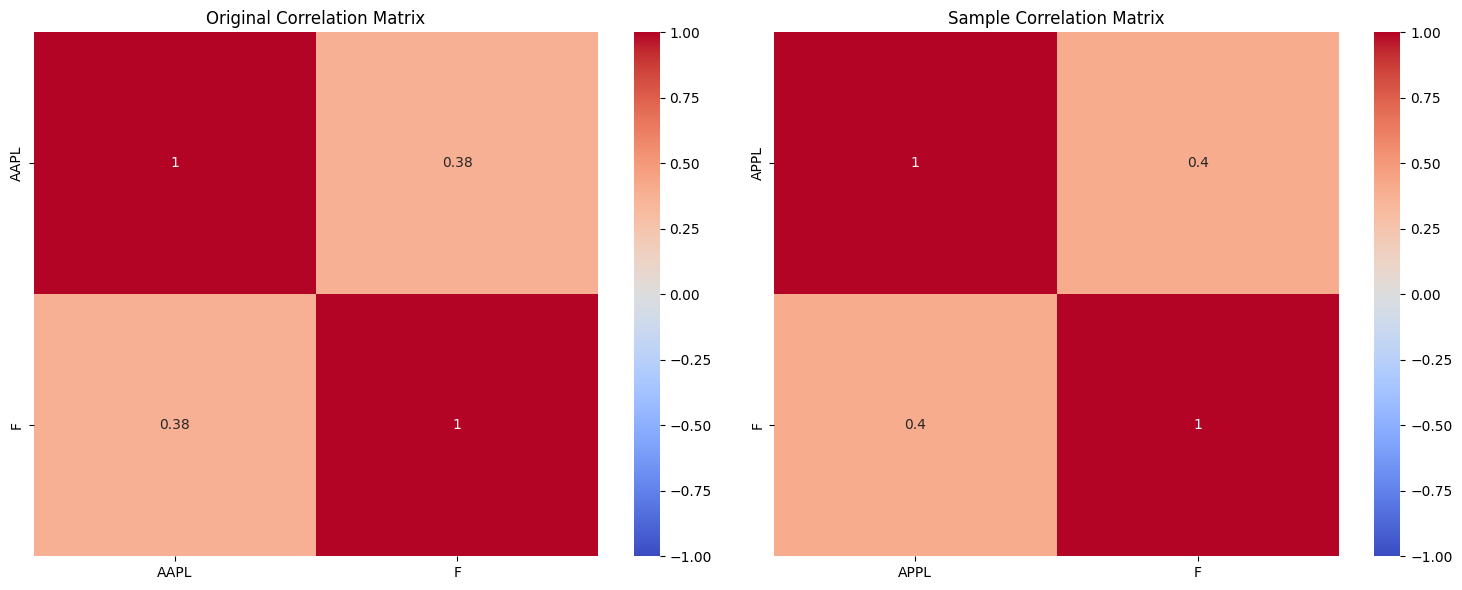
\includegraphics[width=\linewidth,height=0.6\textheight,keepaspectratio]{gfx/m2l3_notes_fig1_plot.png}
\par\smallskip{\small Biểu đồ bài 3}
\end{figure}

\begin{figure}[H]
\centering
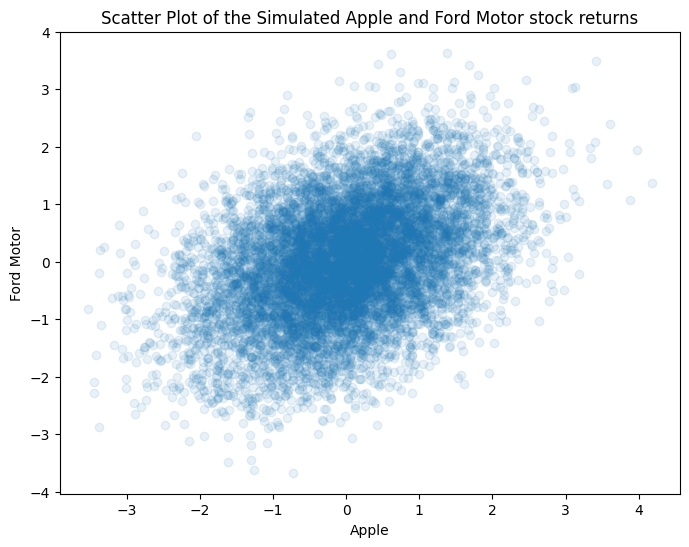
\includegraphics[width=\linewidth,height=0.6\textheight,keepaspectratio]{gfx/m2l3_notes_fig2_plot.png}
\par\smallskip{\small Biểu đồ bài 3}
\end{figure}

Từ ma trận tương quan gốc và ma trận tương quan mẫu ở trên, chúng ta có thể thấy rằng các giá trị tương quan của dữ liệu gốc và dữ liệu được mô phỏng là rất gần nhau.

\section{5. Kết luận}

Trong bài học này, chúng ta đã giới thiệu một vài ma trận đặc biệt và một số công cụ đại số tuyến tính liên quan đến các ma trận này. Chúng ta đã bắt đầu với định nghĩa và các tính chất của một ma trận đối xứng và sau đó là ứng dụng của nó, đặc biệt là dạng đã chéo hóa của nó. Tiếp đó, chúng ta đã mô tả ma trận tam giác trên và ma trận tam giác dưới là gì. Chúng ta chuyển sang các ma trận đối xứng xác định dương và tiếp theo là các ma trận đối xứng bán xác định dương. Chúng ta đã kết thúc bài học bằng việc giới thiệu phân tích Cholesky. Chúng ta đã cung cấp định nghĩa và đi qua một ví dụ bằng số. Chúng ta đã kết thúc phần này với một ứng dụng của phân tích Cholesky bằng mô phỏng Monte Carlo. Tất cả các ma trận đặc biệt này sẽ đóng những vai trò quan trọng trong các công cụ phân tích tài chính mà chúng ta sẽ học trong các bài học tương lai.

\textbf{Tài liệu tham khảo (References)}

\begin{itemize}
  \item Axler, Sheldon. \emph{Linear Algebra Done Right}. 4th edition, Springer, 2024.
\end{itemize}
Copyright 2024 WorldQuant University. This content is licensed solely for personal use. Redistribution or publication of this material is strictly prohibited.
